\documentclass[12pt]{report}
\usepackage{amsthm, amssymb}
\usepackage{geometry}
\geometry{legalpaper, margin=1in}
\usepackage{amsmath}
\usepackage{enumitem}

\newtheorem*{remark}{Remark}
\newtheorem{theorem}{Theorem}
\newtheorem{corollary}{Corollary}[theorem]
\newtheorem{lemma}[theorem]{Lemma}
\newtheorem*{defi}{Definition}
\newtheorem{ex}{Example}
\usepackage{xcolor}
\usepackage{graphicx}

\title{Topology HW 10}
\author{Ben Kallus}
\date{Due Friday, April 30, 2021}

\begin{document}
\maketitle

\medskip\noindent\textbf{1)}

\medskip\noindent\textbf{a)}

    $(\mathbb Q, \cdot)$ is not a group because 0 does not have a multiplicative inverse.

\medskip\noindent\textbf{b)}
\begin{proof}
    Let $a, b \in \mathbb Z$.
    $a+b$ is an integer, so $\mathbb Z$ is closed under $+$.
    Because real number addition is associative, so is $+$.
    Note that $0 + a = a + 0 = a$, so $0$ is the additive identity in $\mathbb Z$.
    Observe that $a + -a = -a + a = 0$.
    Thus, each integer has an additive inverse.
    Therefore, $(\mathbb Z, +)$ is a group.
\end{proof}

\medskip\noindent\textbf{2)}
\begin{proof}
    Let $X$ be a topological space.
    Let $x_0 \in X$, and let $f$ be a loop in $X$ centered at $x_0$.
    In lecture, we showed that the fundamental group of $X$ based at $x_0$ satisfies all the group axioms except for the existence of inverses.
    Thus, to finish the proof, we need only show that there exists a loop $f^{-1}$ such that $[f] * [f^{-1}] = [e]$.
    Define $f^{-1}: [0,1] \to X$ by $$f^{-1}(t) = f(1-t).$$
    Define the $H: [0,1] \times[0,1] \to X$ by $$H(s, t) = \begin{cases} f(2s) & s \in \left[0,\frac{1-t}2\right], \\ f(1-t) & s \in \left[\frac{1-t}2, \frac{1+t}2\right], \\ f^{-1}(2s-1) & s \in \left[\frac{1+t}2,1\right]. \end{cases}$$
    By the Pasting Lemma, $H$ is continuous.
    Thus, because $H(s,0) = f * f^{-1}$ and $H(s,1) = x_0$, $H$ is a path homotopy between $f * f^{-1}$ and $e$.
    Thus, $f * f^{-1} \in [e]$, so $[f^{-1}]$ is the inverse of $[f]$ in the fundamental group of $X$ based at $x_0$.
    Thus, the fundamental group of $X$ is a group.
\end{proof}

\newpage\noindent\textbf{3)}

\medskip\noindent\textbf{a)}

    $x_0 = 0$.
    \begin{center}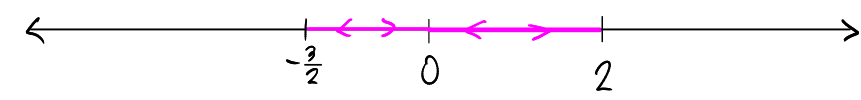
\includegraphics[scale=.6]{1.png}\end{center}
    $\mathbb R$ is simply connected, so there is only one equivalence class of loops based at $x_0$.
    Shown above are two loops based at 0; one travels from 0 to 2 and back, and the other travels from 0 to $-\frac32$ and back.

\medskip\noindent\textbf{b)}

    $x_0 = (1,1)$.
    \begin{center}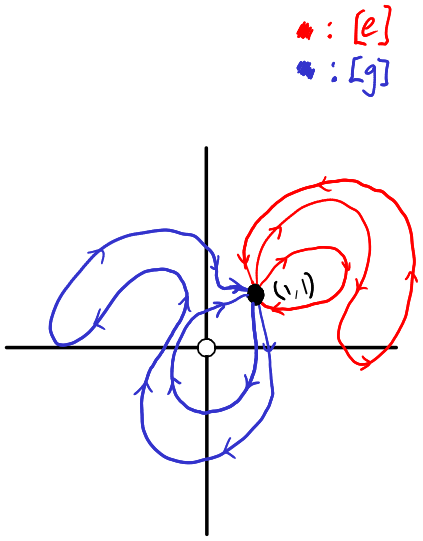
\includegraphics{2.png}\end{center}
    Shown in red are two loops in the identity equivalence class.
    Shown in blue are two loops in the isomorphism class $[g]$.

\newpage\noindent\textbf{c)}

    \begin{center}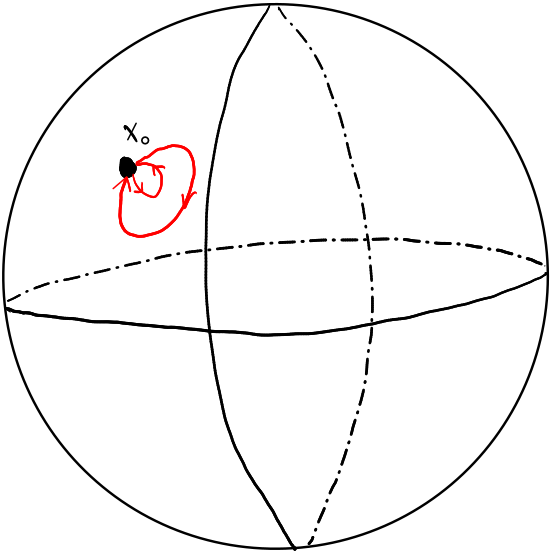
\includegraphics[scale=.6]{3.png}\end{center}
    $S^2$ is simply connected, so there is only one equivalence class of loops centered at $x_0$.
    Shown above are two loops based at $x_0$.

\medskip\noindent\textbf{d)}

\begin{center}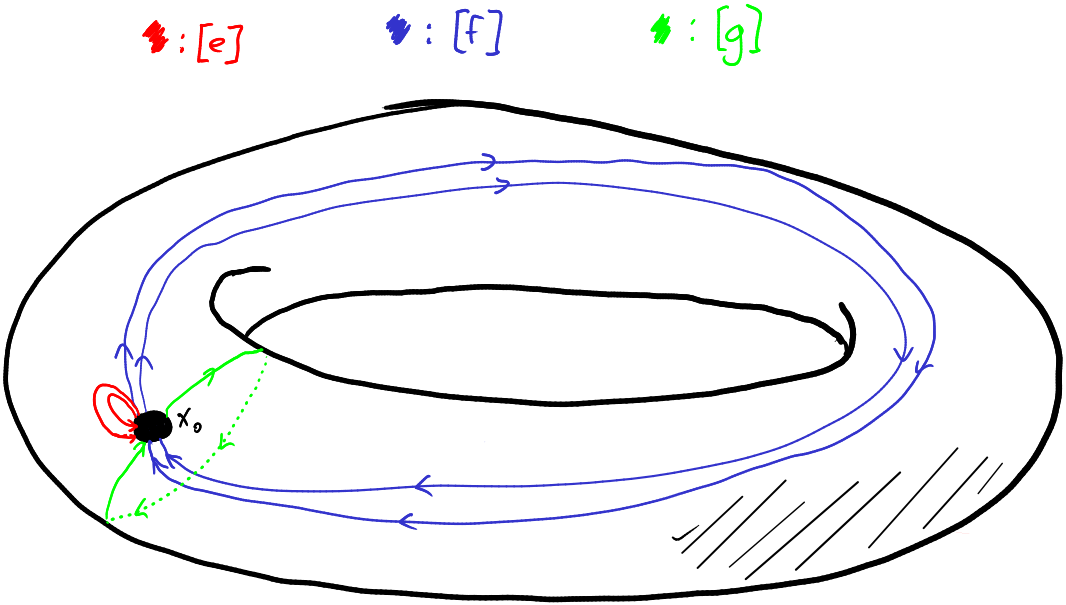
\includegraphics[scale=.5]{4.png}\end{center}
    Shown in red are two loops that are homotopic to the identity.
    Shown in blue are two loops in the equivalence class $[f]$.
    Shown in green is a loop in the equivalence class $[g]$.

\end{document}
